\documentclass[twocolumn, 11pt]{article} % MÅ defineres i ethvert dokument.
\usepackage{longtable}

\usepackage[utf8]{inputenc} %Tillater spesialteikn uten bruk av koding.
\usepackage[norsk]{babel} % Tillater norske teikn.
\usepackage[margin=1in]{geometry} % Definerer marger i dokumentet.
\usepackage{microtype} % Gjør det mer behagelig å lese dokumentet.
\usepackage{amsmath} % Tillater avansert formatering av matte.
\usepackage{amsfonts} % Tillater avanserte teikn, som R for reelle tall.
\usepackage[toc,page]{appendix} 
\usepackage{url}
\usepackage{graphicx} % Tillater mer avansert formatering av grafikk.
\usepackage{geometry} % Tillater enklere formatering av sidevisning.
\usepackage[colorlinks=true, pdfborder={0 0 0}]{hyperref} % Tillater hyperlenker {\href} som under. Colorlinks kan byttes til false hvis man ønsker linker i svart.
\usepackage[tableposition=top]{caption} % Tvinger tabelltekst til å dukke opp over alle tabeller.
\usepackage{graphicx}
\usepackage{float}
\graphicspath{ {./images/} }
\usepackage{listings}
\usepackage{color}
\definecolor{dkgreen}{rgb}{0,0.6,0}
\definecolor{gray}{rgb}{0.5,0.5,0.5}
\definecolor{mauve}{rgb}{0.58,0,0.82}
\lstset{frame=tb,
  language=Python,
  aboveskip=3mm,
  belowskip=3mm,
  showstringspaces=false,
  columns=flexible,
  basicstyle={\small\ttfamily},
  numbers=none,
  numberstyle=\tiny\color{gray},
  keywordstyle=\color{blue},
  commentstyle=\color{dkgreen},
  stringstyle=\color{mauve},
  breaklines=true,
  breakatwhitespace=true,
  tabsize=1
}

%I enkelte laboratorieoppgaver kan det bli nødvendig å laste flere pakker. Ta internett (deriblant lenkene nedafor) til hjelp i søket etter rett pakke. Noen har sannsynligvis lurt på det samme som deg.
\begin{document}

\twocolumn[
  \begin{@twocolumnfalse}
\textbf{
  \title{Principal Component Analysis}
  \author{Bård Tollef Pedersen og Erik Lykke Trier}
  \date{22. januar 2023} % \today gir dagens dato
  \maketitle
} 
\begin{center}
Laget i \LaTeX.
\end{center}
    \begin{abstract}
    \begin{large}
    \

    Formålene med denne analysen er å finne ut om det er en sammenheng mellom PCA og regime type, og PCA og kontinent, i tillegg skulle gruppen undersøke om det fantes andre korrelasjoner. Dataene er samlet fra Wikipedia og gitt av oppgaveteksten \cite{oppgavetekst}. Gruppen fant ut at man kan bruke PC1 og PC2 for å skille regimetypene, men ikke til å skille kontinenter. Gruppen sjekket om det var en korrelasjon mellom registrert og uregistrert alkoholforbruk i forhold til regime type, gruppen konkluderte med at det ikke er en korrelasjon her. 
    
    \end{large}
    \end{abstract}
  \end{@twocolumnfalse}     
  ]
\section{Innledning} 
    PCA er en statistisk metode for å sammenligne og analysere data. Denne metoden blir blant annet også brukt for finne korrelasjoner i data. Når en gjennomfører en PCA kan man bruke programmer for å gjøre denne jobben lettere, ett av de er Quasar. Det var dette programmet gruppen brukte i analysen.
    
    I denne rapporten tar gruppen for seg en PCA av forskjellige variabler for å se etter korrelasjoner og sammenhenger. Mer nøyaktig sammenligner gruppen styremåte med registrert alkohol forbruk og uregistrert alkohol forbruk for å se om det er korrelasjon.

    
\section{Teori og metoder}
\subsection{Principal Component Analysis}
\textit{Principal Component Analysis} eller PCA er en statistisk metode for å analysere og redusere dimensjonalitet i et datasett. Det gjør dette ved å finne de viktigste komponentene, de komponentene som gir mest mulig variasjonsdekning i datasettet. PCA kan også brukes til å visualisere dataene i et lavere dimensjonsrom ved hjelp av et spredningsplott, dette kan være nyttig for å identifisere mønstre eller uteliggere i dataene.\cite{youtube} Før en PCA ble datene normalisert ved å dele verdiene på standardavviket deres. Dette gjøres for at dataene som har veldig høye tall ikke skal dominere sammenhengene. 

\subsection{Orange/Quasar}
Orange er et verktøysett for datavisualisering, maskinlæring og datautvinning. Den har et visuelt programmeringsvindu, som vist i figur \ref{Oppsett_quasar}. Dette gjør at en rask kan gjennomføre kvalitativ dataanalyse og datavisualisering.\cite{Orange}

Quasar er et \textit{open source} prosjekt, som er en samling av dataanalyseverktøy en bruker til å utvide Orange-pakken\cite{Quasar}. Verktøyet gjør det veldig lett å prosjektere data ved hjelp av PCA og spredningsplot. 

\begin{figure}[ht]
\includegraphics[width=0.49\textwidth]{images/Oppsett_quasar.jpg}
\caption{Skjermbilde av oppsett i programmet Quasar.}
\label{Oppsett_quasar}
\end{figure}

Oppsettet som ble brukt for å komme fram til resultatene er vist i figur \ref{Oppsett_quasar}. 
Starter med \textit{CSV file import} hvor en legger inn all dataene. Videre drar man en tråd fra \textit{CSV file import} blokken til \textit{Data Table}. \textit{Data Table} gjør om på filen, fra en csv-fil til en tabell. Dette gjør det lettere for både programmet og brukeren å jobbe videre med dataene. Fra \textit{Data Table} drar man en ny tråd til \textit{Select Columns}. \textit{Select Columns} gjør at en kan velge hvilke variabler som skal bli brukt og ignorert. Videre trekker man en tråd til PCA. Her velger man hvor mange komponenter en vil bruke til plotting og analyse. Gruppen valgte å bruke to komponenter. Etterfulgt av PCA kan en se at det er trekt tråd til både \textit{Scatter Plot} og \textit{Save Data}. \textit{Save Data} brukes for å lagre og plotte ladningsplott i Excel. Excel ble brukt ettersom Quasar ikke har en bra ladningsplott funksjon. \textit{Scatter Plot} blokken er der en plotter og viser hovedkomponentene mot hverandre. 

\subsection{Datasett}
Datasettet som har blitt brukt i dette forsøket inneholder 18 forskjellige komponenter og er registrert per land. De 18 komponentene er: registrert alkoholforbruk, uregistrert alkoholforbruk, andel alkohol konsumert i øl, andel alkohol konsumert i vin, andel alkohol konsumert i sprit, alkohol konsumert i andre alkohol holdige drikker, demokrati skår, valgprosess, hvor funksjonelt demokratiet er, politisk deltakelse, politisk kultur, sivile rettigheter, brutto nasjonal produkt per innbygger, kriminell frekvens, totalt antall kriminelle handlinger, regime type og kontinent.

Gruppen valgte og lage en PCA med to hovedkomponenter, PC1 og PC2, disse komponentene beskriver 66\% av all dataene.

Datasettet ble gitt i oppgaven og stammer fra forskjellige Wikipedia sider som det ligger lenker til i oppgave teksten \cite{oppgavetekst}.  



\section{Resultater}

Resultatet av PC1 og PC2 plottet som x og y-aksen kan sees i figur \ref{PCA_Regimetype} og \ref{PCA_Kontinent}. I figur \ref{PCA_Regimetype} brukes fargene for å skille de forskjellige regime typene, mens i figur \ref{PCA_Kontinent} brukes fargene for å skille de forskjellige kontinentene.

\begin{figure}[H]
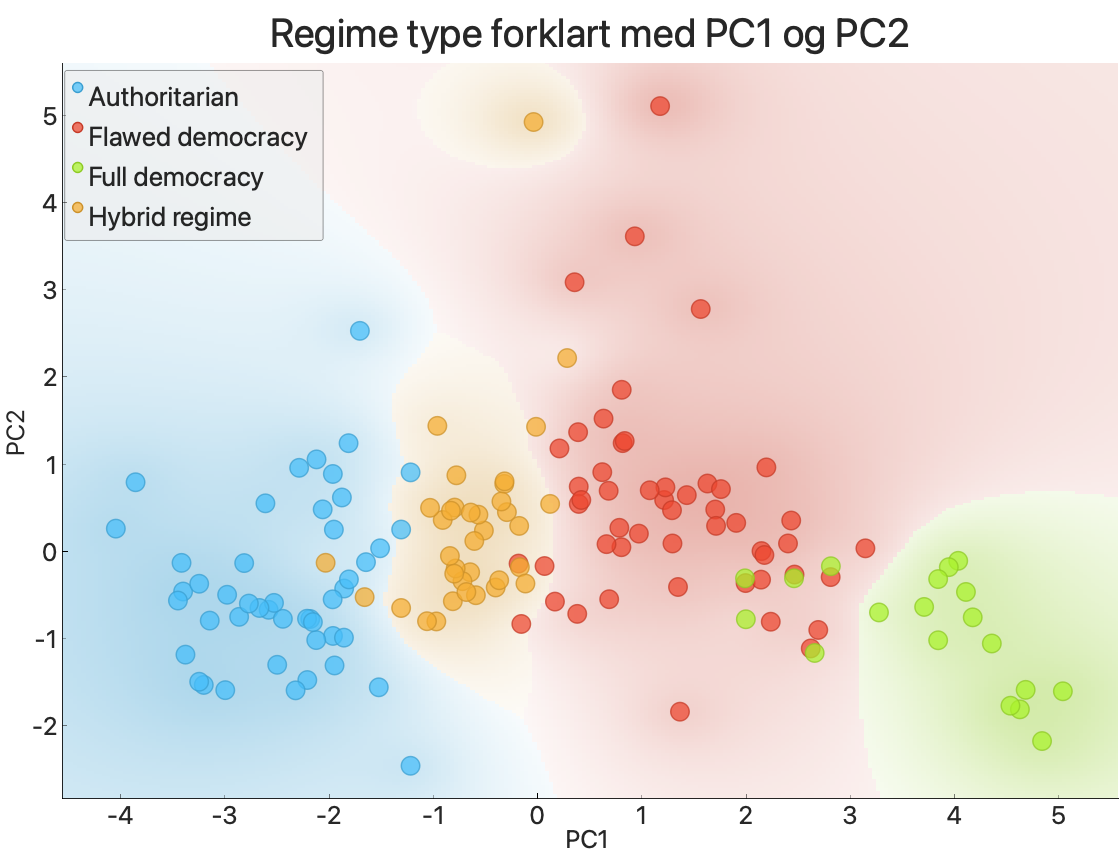
\includegraphics[width=0.5\textwidth]{images/PCA_Regimetype.png}
\caption{I plottet ser man PC1 som x-aksen, PC2 som y-aksen og farge definerer de forskjellige regime typene}
\label{PCA_Regimetype}
\end{figure}

\begin{figure}[H]
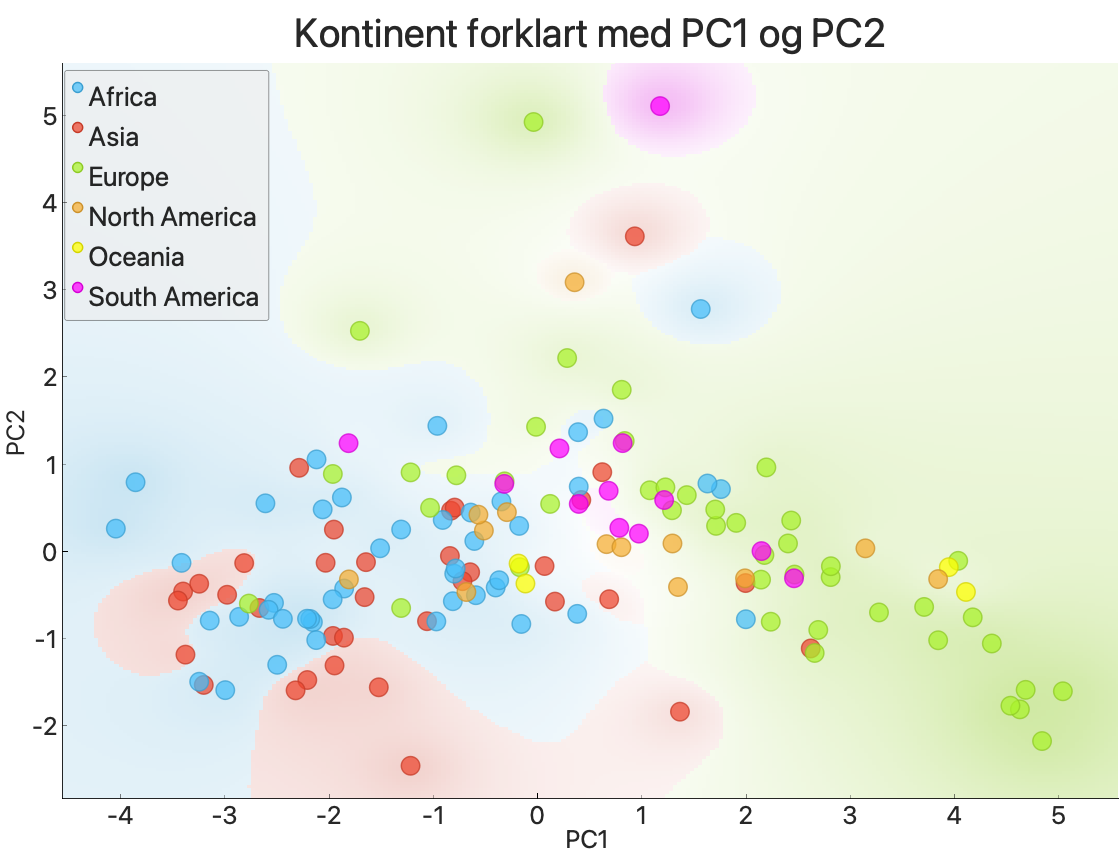
\includegraphics[width=0.5\textwidth]{images/PCA_Kontinent.png}
\caption{I plottet ser man PC1 som x-aksen, PC2 som y-aksen og farge definerer de forskjellige kontinentene typene}
\label{PCA_Kontinent}
\end{figure}

I figur \ref{loading_pc1} og \ref{loading_pc2} kan en se ladningsplottene til de to hovedkomponentene, PC1 og PC2. Her kan en lett se hvilke variabler som blir vektet mest med de forskjellige hovedkomponentene.

\begin{figure}[H]
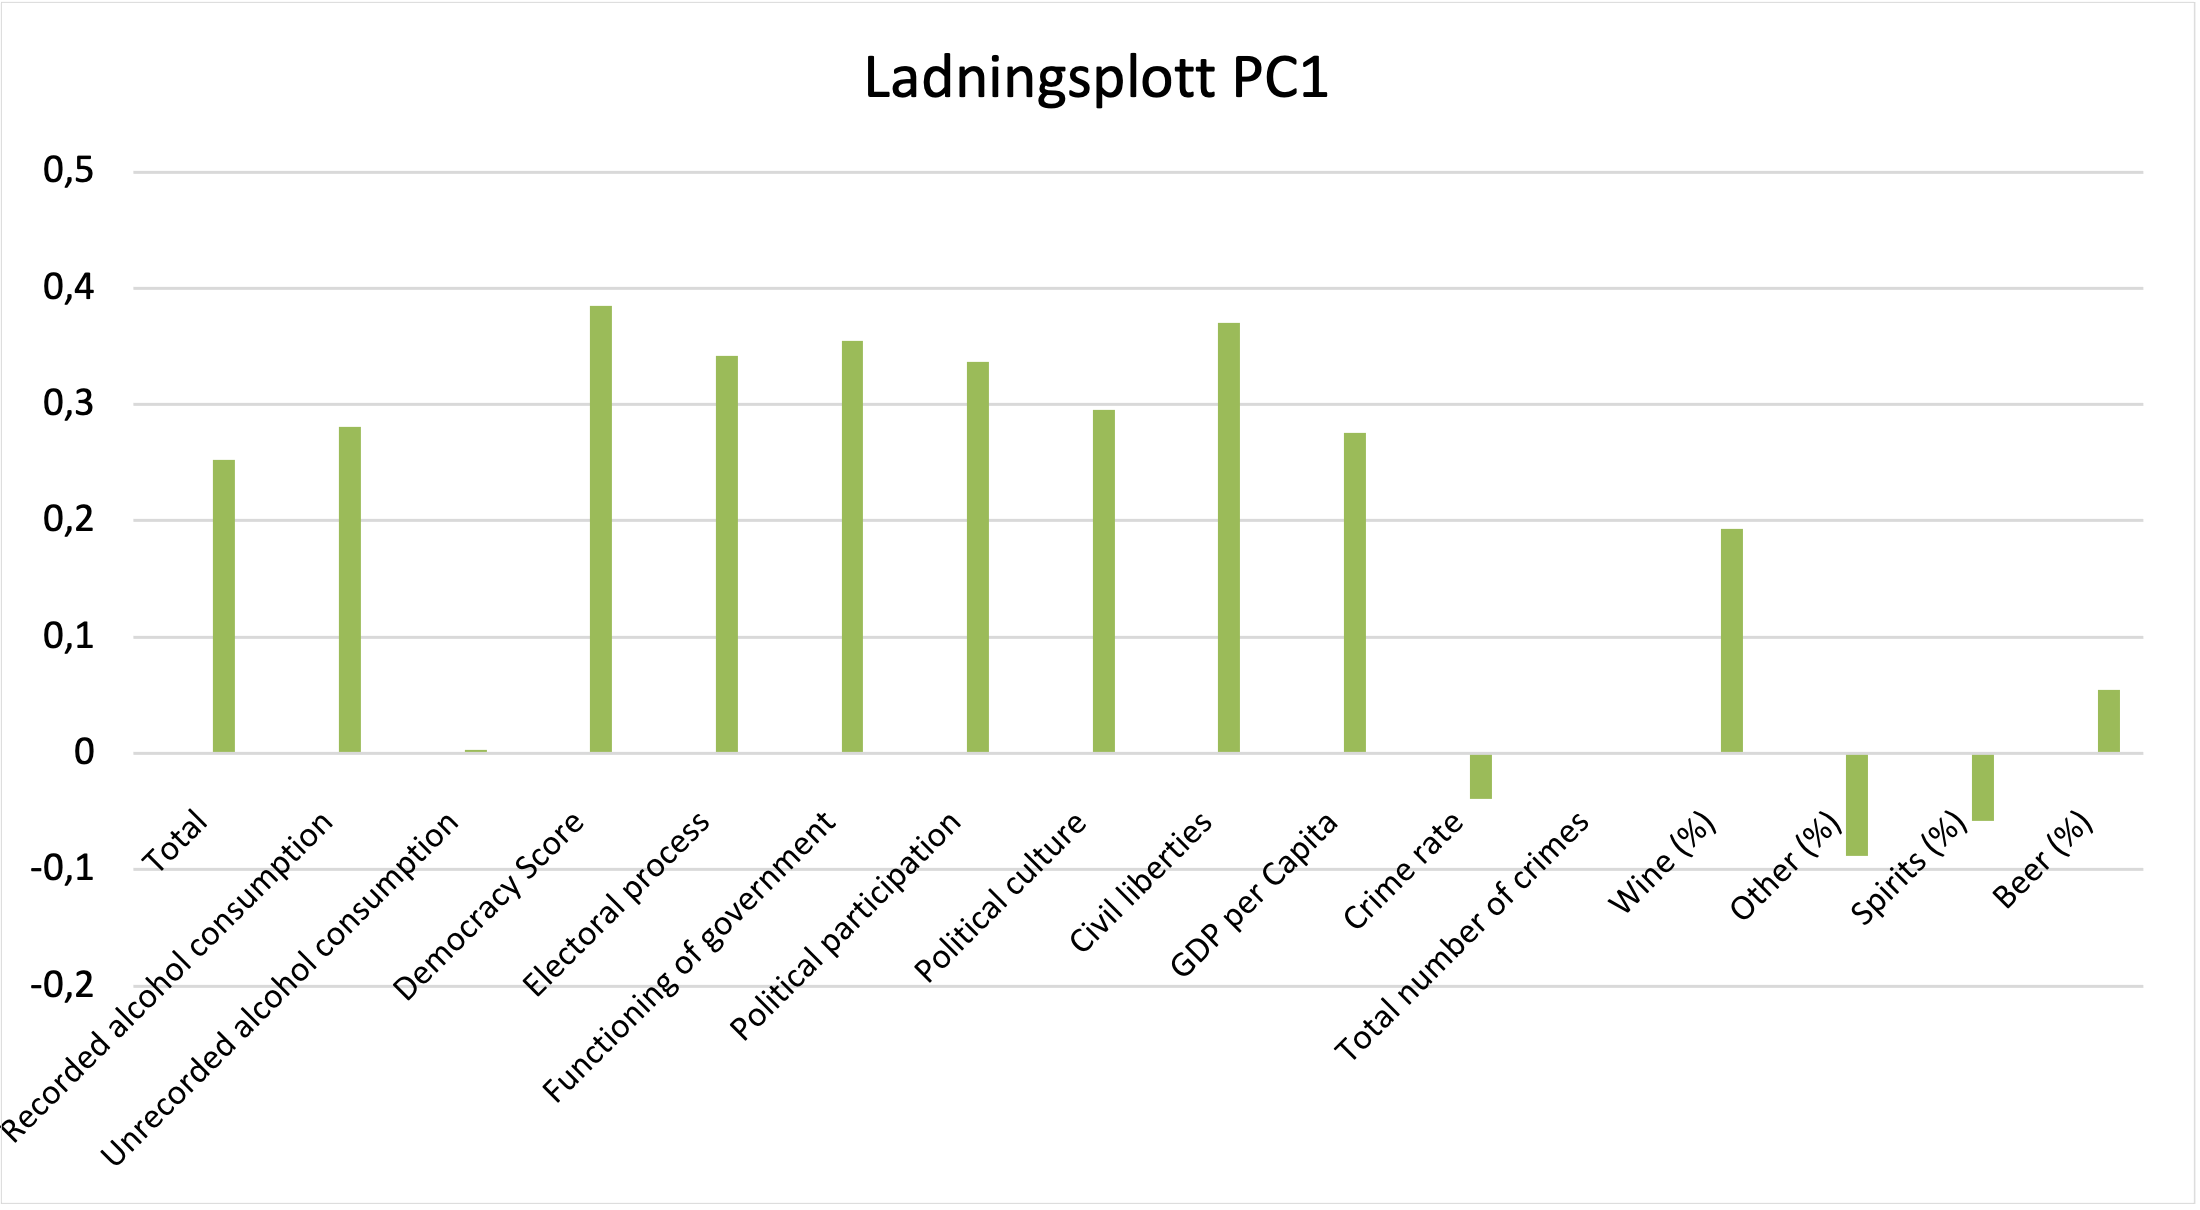
\includegraphics[width=0.5\textwidth]{images/Ladningsplott_pc1.png}
\caption{I plottet ser vi loading plot av PC1 som viser hvilke variabler PC1 er satt sammen av og hvor mye hver komponent teller.}
\label{loading_pc1}
\end{figure}

\begin{figure}[H]
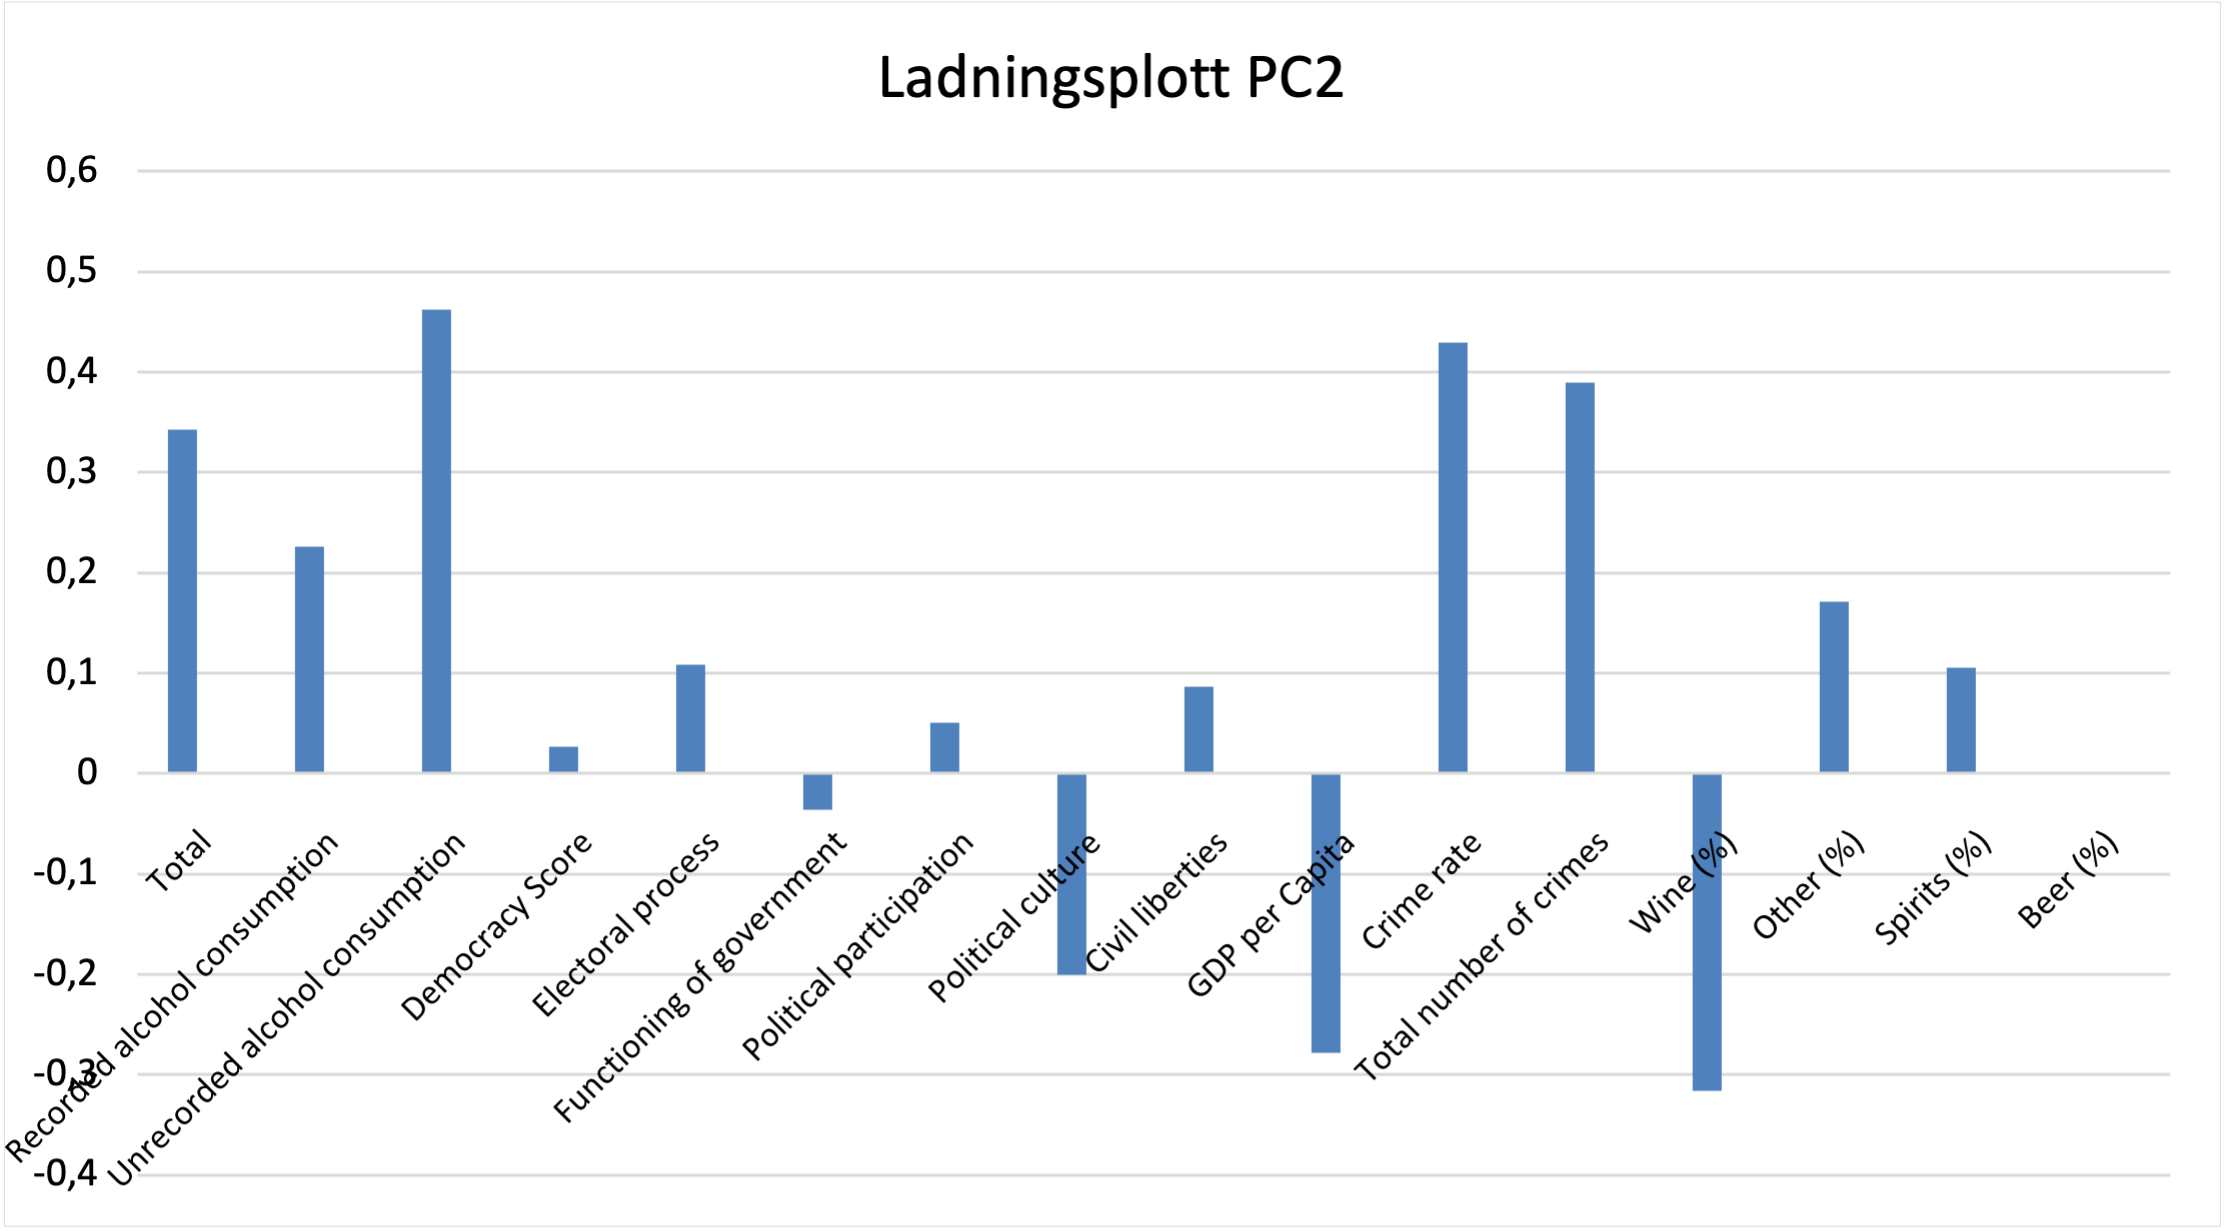
\includegraphics[width=0.5\textwidth]{images/ladningsplott_pc2.png}
\caption{I plottet ser man loading plot av PC2 som viser hvilke variabler PC2 er satt sammen av og hvor mye hver komponent teller.}
\label{loading_pc2}
\end{figure}


I figur \ref{Registrert_alkoholforbruk} og \ref{Uregistrert_alkoholforbruk} har gruppen plottet alkohol forbruk med demokrati-indeks. Der figur \ref{Registrert_alkoholforbruk} er plottet med registert alkohol forbruk og figur \ref{Uregistrert_alkoholforbruk} er plottet med uregistrert alkohol forbruk. Dette var også det eneste gruppen fant av sammenhenger mellom datene.

\begin{figure}[H]
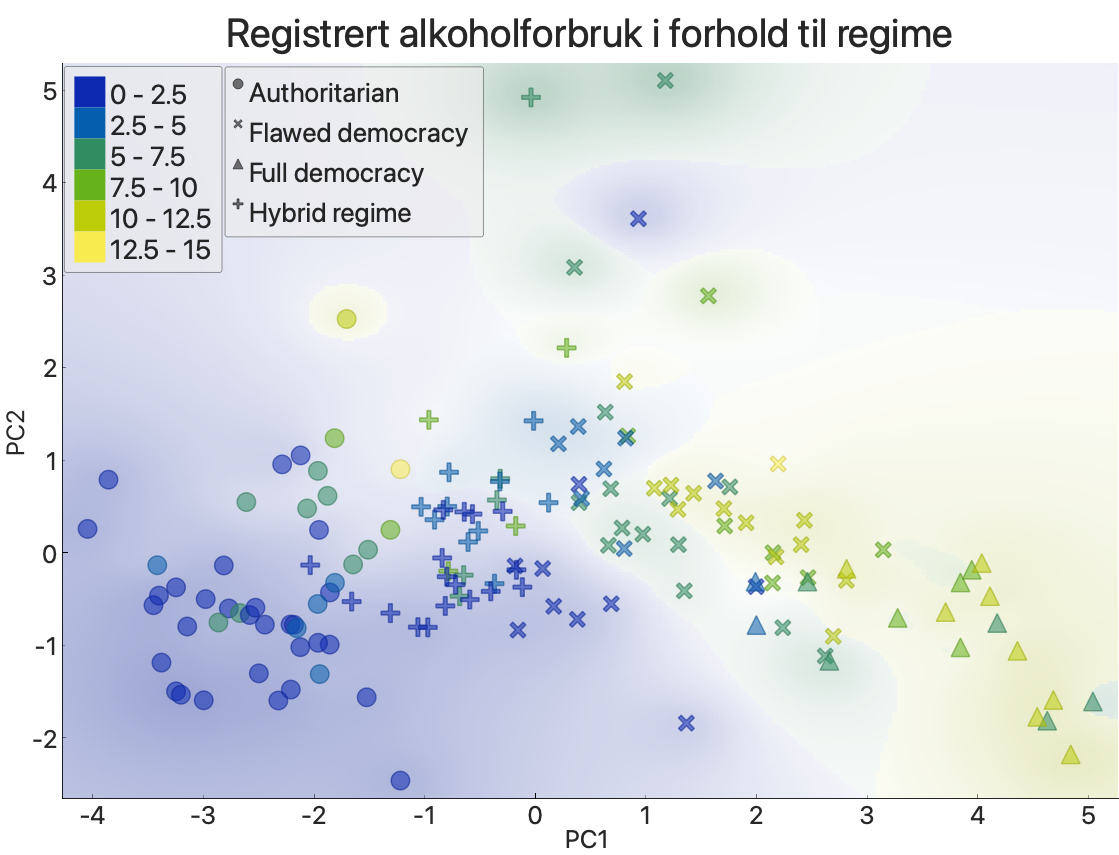
\includegraphics[width=0.5\textwidth]{images/Registrert_alkoholforbruk.png}
\caption{I plottet ser man PC1 som x-aksen, PC2 som y-aksen og farge definerer registrert alkoholforbruk i liter, de forskjellige tegnene representerer de forskjellige regime typene}
\label{Registrert_alkoholforbruk}
\end{figure}

\begin{figure}[H]
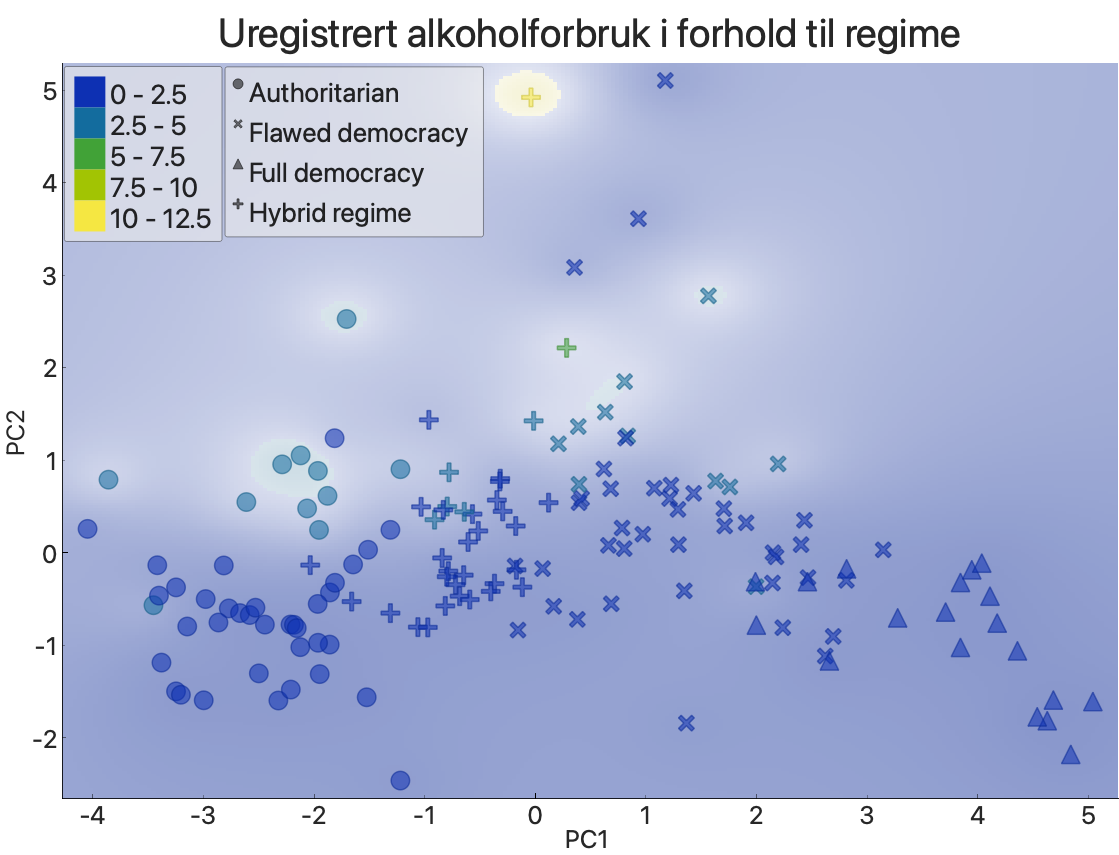
\includegraphics[width=0.5\textwidth]{images/Uregistrert_alkoholforbruk.png}
\caption{I plottet ser man PC1 som x-aksen, PC2 som y-aksen og farge definerer uregistrert alkoholforbruk i liter, de forskjellige tegnene representerer de forskjellige regime typene}
\label{Uregistrert_alkoholforbruk}
\end{figure}

\section{Diskusjon}

Det som skulle sjekkes med figur \ref{PCA_Regimetype} og \ref{PCA_Kontinent} er om en kan tydelig gruppere dataene etter kontinent eller regime type ved hjelp av PCA plottet. 

I figur \ref{PCA_Regimetype} kan en tydelig se en gruppering. Her ligger land med høy demokrat-indeks langt til høyre og land med lav indeks langt til venstre. Det betyr at mye av PC1 kan forklares med demokrat-indeksen. Dette stemmer også overens med figur \ref{loading_pc1} hvor en kan se at PC1 er forklart mye med demokrati-indeksen.
For figur \ref{PCA_Kontinent} er det ikke særlig tydelige grupperinger. I midten er det en veldig god blanding fra alle kontinentene. Nederst til venstre kan man se en liten samling av europeiske land, men det er fremdeles mange europeiske land i andre deler av plottet så de europeiske landene er ikke eksklusivt langt til høyre. Det er også en liten samling asiatiske land alene i nedre venstre del av plottet, men de er heller ikke eksklusivt der, så man kan se på de som uteliggere fra normalen. 

En annen mulig sammenheng som ble presentert i resultatdelen av rapporten er mellom registrert alkoholforbruk og regime typer. I figur \ref{Registrert_alkoholforbruk} ser en registrert alkoholforbruk i farge spekteret og regime typene har fått hver sin fasong. Det er en antydning til en trend her. Som man ser på bakgrunnsfargene så går det fra lavere alkoholbruk ved lav PC1 verdi til høyere alkohol forbruk ved høy PC1 verdi. Dette stemmer også overens med ladningsplottet til PC1, figur \ref{loading_pc1}. Det er også en antydning til høyere frekvens av demokratiske land ved høy PC1 verdi. Det er derfor tegn til korrelasjon mellom registrert alkoholforbruk og regimetype. Høyre demokrati-indeks har en korrelasjon til høyre alkohol forbruk. Ettersom det bare er tegn og ikke fullstendige gruppering kan man ikke konkludere med at det er en fullstendig korrelasjon mellom registrert alkoholforbruk og regimetype.

På figur \ref{Uregistrert_alkoholforbruk} vises uregistrert alkoholforbruk i forhold til de forskjellige regimene og her skårer alle lavt untatt en uteligger som er Moldova som viker tydelig fra trenden. Dette kan være fordi det er jevnt lite uregistrert alkoholforbruk, men også fordi dette bare er antakelser og ikke nøyaktig data.
Uregistrert alkoholforbruk er estimat satt sammen av spørreundersøkelse og antagelser av eksperter \cite{oppgavetekst}. Dette gjør dataene usikker og mindre troverdig.

\bigskip

Ettersom oppgaven er å finne korrelasjoner mellom de forskjellige komponentene i datasettet, er det lett å se korrelasjoner der de ikke eksisterer. Dette er fordi man vil gjerne finne en korrelasjon. Det kan skje da at man heller finner en svak trend som man over bedømmer som en korrelasjon når det egentlig bare er en tilfeldighet eller liknende. 

Fordi gruppen valgte å bare se på to hovedkomponenter er ikke all data beskrevet. I dette tilfelle ble 66\% av dataene forklart med to hovedkomponenter. I dataene som ikke er med kan det vare sammenhenger eller mønstre. Ettersom majoriteten av dataene er representert fra de to hovedkomponentene er sannsynlighet for å finne korrelasjoner blant resten liten.


\section{Konklusjon}
En kan bruke PC1 og PC2 for å skille de forskjellige styremetodene. Dette kan en enkelt se fra figur \ref{PCA_Regimetype} hvor alle de forskjellige styremåtene er gruppert. Dette kan også bekreftes med figur \ref{loading_pc1} hvor en ser at demokrati-indeksen har et stort bidrag til PC1. 
En kan ikke bruke PC1 og PC2 for å skille de forskjellige kontinentene, ettersom det er for mye spredning i figur \ref{PCA_Kontinent}. 

I figur \ref{Registrert_alkoholforbruk} kan en se tilnærming til en korrelasjon, men det er for mange uteliggere til at man kan konkludere med at det er en sammenheng. I figur \ref{Uregistrert_alkoholforbruk} kan en se at det er null korrelasjon mellom uregistrert alkoholforbruk og styre metode. 


\bibliographystyle{plain}
\bibliography{sources2.bib}

\end{document}

